\documentclass[tikz,border=3pt]{standalone}
\usepackage{pgfplots}
\usepgfplotslibrary{groupplots}
\pgfplotsset{compat=1.18}
\definecolor{oiBlue}{HTML}{0072B2}
\definecolor{oiOrange}{HTML}{E69F00}
\definecolor{oiGreen}{HTML}{009E73}
\definecolor{oiRed}{HTML}{D55E00}
\begin{document}
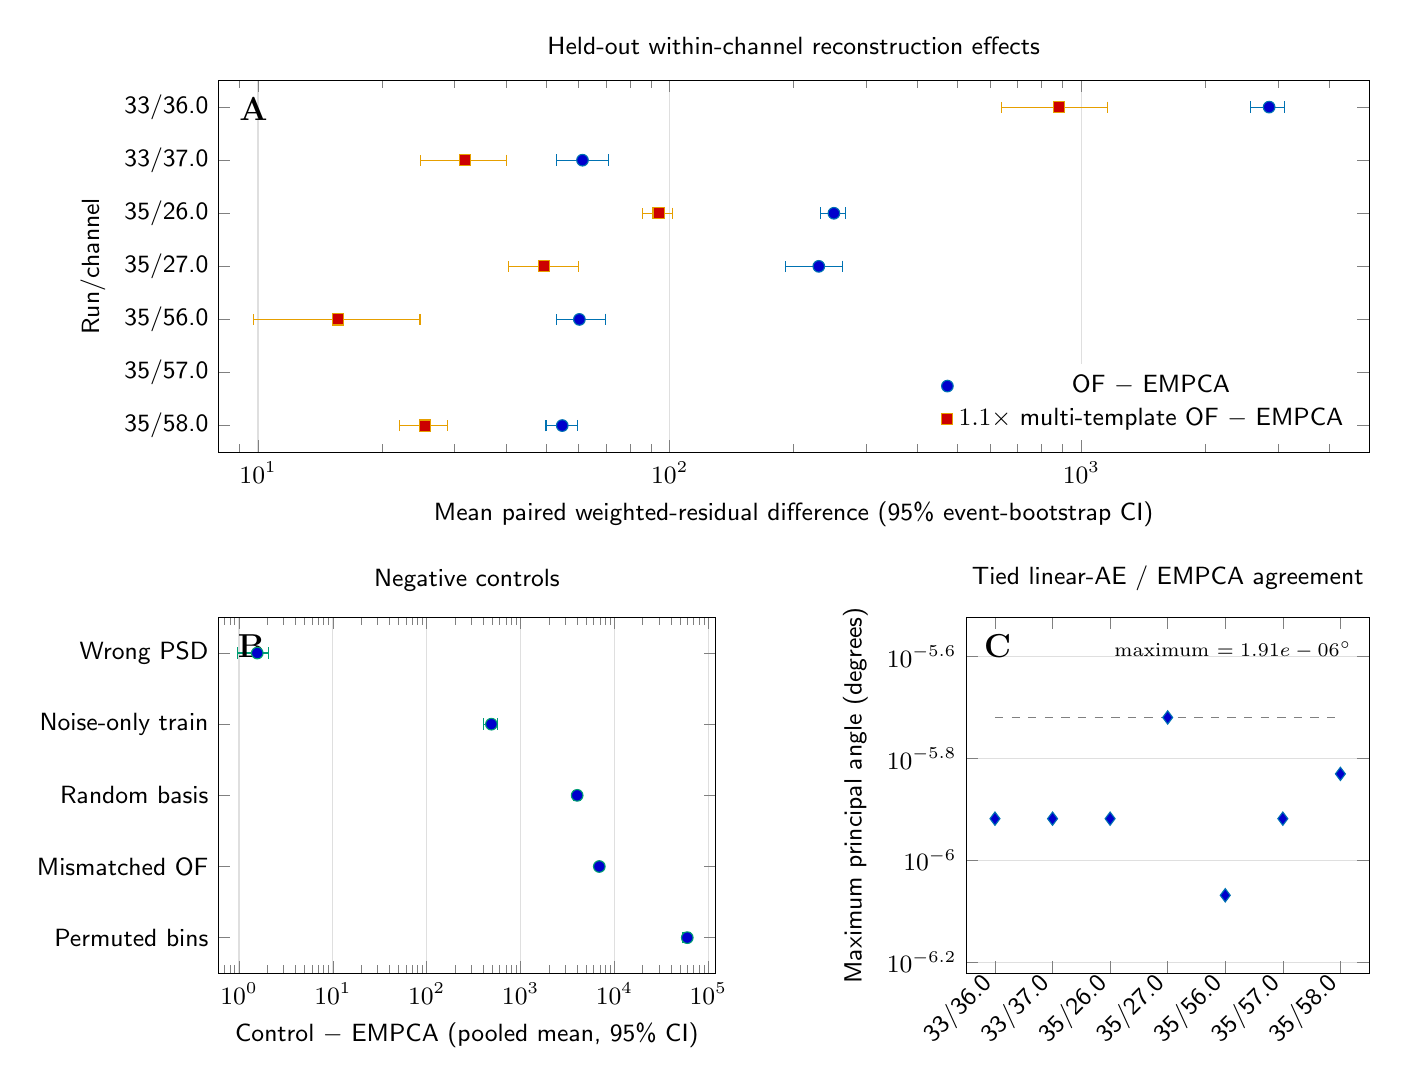
\begin{tikzpicture}[font=\sffamily\small]
\begin{axis}[
  name=top, width=16.2cm, height=6.3cm,
  xmode=log, xmin=8, xmax=5000,
  ymin=-0.5, ymax=6.5, y dir=reverse,
  ytick={0,1,2,3,4,5,6}, yticklabels={{33/36.0},{33/37.0},{35/26.0},{35/27.0},{35/56.0},{35/57.0},{35/58.0}}, ylabel={Run/channel},
  xlabel={Mean paired weighted-residual difference (95\% event-bootstrap CI)},
  title={Held-out within-channel reconstruction effects},
  xmajorgrids, grid style={gray!25},
  legend style={draw=none, at={(0.99,0.03)}, anchor=south east},
  error bars/x dir=both, error bars/x explicit,
]
\addplot+[only marks, mark=*, mark size=2.1pt, oiBlue, error bars/.cd, x dir=both, x explicit]
table[x index=0, x error minus index=1, x error plus index=2, y index=3] {
2856.8610746 281.476545461 257.198274912 0
61.3871193523 8.39422870652 9.45392280549 1
250.471337718 17.6711003264 16.3440513547 2
230.155320413 38.6335339294 32.9590870002 3
60.3306031448 7.35141773769 9.39807490581 4
1609.10316111 162.133781301 180.801687619 5
54.8153824619 4.76632916616 4.93504798862 6
};
\addlegendentry{OF $-$ EMPCA}
\addplot+[only marks, mark=square*, mark size=2.0pt, oiOrange, error bars/.cd, x dir=both, x explicit]
table[x index=0, x error minus index=1, x error plus index=2, y index=3] {
882.185819776 242.073665239 275.825333079 0
31.8213657296 7.03062602775 8.2664008882 1
93.929056649 7.96048184401 7.548579052 2
49.5705639066 8.90013264589 10.3457228116 3
15.6112140618 5.87201803687 9.13214349515 4
856.254017419 167.281773663 173.508411135 5
25.448604436 3.38198723576 3.4121005688 6
};
\addlegendentry{$1.1\times$ multi-template OF $-$ EMPCA}
\node[anchor=north west, font=\bfseries\large] at (rel axis cs:0.01,0.98) {A};
\end{axis}

\begin{axis}[
  at={($(top.south west)+(0,-2.1cm)$)}, anchor=north west,
  width=7.9cm, height=6.1cm,
  xmode=log, xmin=0.6, xmax=120000,
  ymin=-0.5, ymax=4.5, y dir=reverse,
  ytick={0,1,2,3,4}, yticklabels={{Wrong PSD},{Noise-only train},{Random basis},{Mismatched OF},{Permuted bins}},
  xlabel={Control $-$ EMPCA (pooled mean, 95\% CI)},
  title={Negative controls}, xmajorgrids, grid style={gray!25},
  error bars/x dir=both, error bars/x explicit,
]
\addplot+[only marks, mark=*, mark size=2.1pt, oiGreen, error bars/.cd, x dir=both, x explicit]
table[x index=0, x error minus index=1, x error plus index=2, y index=3] {
1.56741869153 0.593132095372 0.511249124981 0
489.401256874 83.816637891 74.4999923957 1
4013.47261312 318.707330293 290.920209283 2
6911.8244483 345.126538364 329.383982184 3
59812.7172892 5898.690445 5266.7386103 4
};
\node[anchor=north west, font=\bfseries\large] at (rel axis cs:0.02,0.98) {B};
\end{axis}

\begin{axis}[
  at={($(top.south west)+(9.5cm,-2.1cm)$)}, anchor=north west,
  width=6.7cm, height=6.1cm,
  ymode=log, ymin=6e-7, ymax=3e-6,
  xmin=-0.5, xmax=6.5, xtick={0,1,2,3,4,5,6}, xticklabels={{33/36.0},{33/37.0},{35/26.0},{35/27.0},{35/56.0},{35/57.0},{35/58.0}},
  x tick label style={rotate=45, anchor=east},
  ylabel={Maximum principal angle (degrees)},
  title={Tied linear-AE / EMPCA agreement},
  ymajorgrids, grid style={gray!25},
]
\addplot+[only marks, mark=diamond*, mark size=2.4pt, oiBlue]
table[x index=0, y index=1] {
0 1.20741826973e-06
1 1.20741826973e-06
2 1.20741826973e-06
3 1.90909591042e-06
4 8.53773646252e-07
5 1.20741826973e-06
6 1.47877933347e-06
};
\addplot+[gray, dashed, mark=none] coordinates {(0,1.90909591042e-06) (6,1.90909591042e-06)};
\node[anchor=north east, font=\scriptsize] at (rel axis cs:0.98,0.96)
  {maximum $= 1.91e-06^\circ$};
\node[anchor=north west, font=\bfseries\large] at (rel axis cs:0.02,0.98) {C};
\end{axis}
\end{tikzpicture}
\end{document}
